%1234567890123456789012345678901234567890123456789012345678901234567890123456789
\chapter{Introduction}

The human desire to be physically impressive has a long history which can be
dated back to ancient Greece.
The ancient Olympic Games celebrated the glory of physical dominance of
athletic strength and agility, to achieve the goals faster and more
effortlessly. 
In modern days, physical agility continue to captivate our imagination in
various areas, such as sports, entertainments, or robots.
In the film or game industries, agile motions are important contents to make
their games or movies more fun and entertainings, from an iconic game
Prince of Persia [PP] to a recent big hit animation, Frozen [FR].
Besides entertainment values, being agile and strong also holds great practical
values, such as recovering disaster scenes with robots.
When there was a nuclear melt down that was too dangerous to be recovered
by human due to high radiation levels, few robots were entered to measure
temperature and radioactivity but failed due to limited speed and range of
operations [WIKIPEDIA].
Although even the state-of-arts humanoids are not as agile as human athelets
or virtual characters in animations, their software and hardware specification
have made substantial progress in past few dacades and will have enough agility
to execute athletic motor skills in near future.

Although the word ``agile'' has similar meaning in everyone's mind,
it needs a more clear definition to be discussed in this dissertation.
According to many dictionaries [DICT], the language definition of ``agile''
is ``able to move quickly, easily, effortlessly, and gracefully.''.
It is more straightforward to associate a concrete physical meaning to the
first word ``quickly'' because its meaning can be directly mapped into
high momentum.
However, the other descriptors, ``easily'', ``effortlessly'', and
``gracefully'' are more difficult to be translated because they can be due to
different reasons, such as the innate strengh of the subject, the accumulated
experience, or the ability to negotiate with the environment.
Instead of this loose verbal definition, I will use a narrow definition of the
word ``agile'' in the context of motions, ``able to move quickly and
effortlessly in a complex environment.'', which highlights torque efficiency
and well-coordinated strategies that exploits the environment.
Great examples of agile motions are motor skills of Parkour, such as
vaults, jumps, or flips which are developed to move from the current location
to destination in the most efficient path.
Those skills are well aligned with the previous definition because they are
executed with high linear and angular momentum, and planned to negotiate
environmental features such as walls, guard rails, or stairs. 

The aim of this dissertation is to design a set of computational tools to
develop agile motor skills on virtual and real humanoids.
Although the grand goal would be to achieve agile motor skills on humanoid
robots, but there are many unsolved practical issues to directly design aigle
motions on the hardware, such as delays, noises, or safety concerns.
Especially unlike biped walking where adequate models and control theories are
already available, agile motions have not been studied extensively in the
literature of computer animation and robotics.
Thefore, the appropriate approach toward agile real humanoids is to first
develop theoretical models and control algorithms on the physics-based
simulation where researchers in compter graphics can accomplish complex and
stunning tasks, and then transfer the solution to the real hardware
with the careful adjustment.
Although there are intrinsic differences between virtual and real systems on
models, sensors, actuators, and so on, simulation-developed solutions will
greatly reduce the expensive cost of hardware experiments and prevent
unexpected dangerous situations.

Agile motor skills are difficult tasks for humanoids.
General characteristics of agile motions, high momentum or frequent changes
of contacts, increase difficulties of most existing issues in motor control
problems tremendously.
For instance, simple motion trajectories that are developed in virtual
simulation are more likely not to work on physical systems
because small errors can be quickly accumulated and result drastic deviations
from the original agile motions.
On the top of existing issues, agile motions generate few unique challenges
need to be addressed.
Unlikely well-defined motions such as running or reaching, agile motions cover
a wide range of diverse skills, such as jumping, vaulting, or rolling which are
governed by different control mechanisms and principals.
Because it is infeasible to manually design controllers for all tasks, we want
to develop a set of general tools for learning a variety of agile motions.
In addition, safety of humanoids must be ensured by learning how to fall
both intentionally and inadvertently, which are fundamental motor skills
required by various agile motions. 
These additional, unique challenges motivated me to address following problems
in this dissertation, as steps to achieve agile motions on virtual and real
humanoids.

\section{Falling Strategies for Humanoids}
% Introduction on the falling - Motivation, Description, Goal
Falling and landing motions are a set of fundamental motor skills
in various agile motions to protect humanoids themselves.
Because atheletic movements frequently involves
transitions between airborne and contact phases, they must know how to
absorb the shock at the landing moment and avoid damage to the body parts.
In addition, well-executed falling motions will lead a smooth transition to the
next motor skill. 
In this dissertation, I will discuss two different scenarios of fallings, 
for  virtual and real humanoids.
For a virtual humanoid, I will describe a physics-based controller that allows
the character to fall from a wide range of heights and initial speed, 
which are inspired by agile falling and landing of Parkour practioners.
For a real humanoid, I wiill propose a falling strategy for managing unexpected
falls due to a wide range of perturbations.
The effectiveness of both presented strategies are validated by measuring
amounts of joint stresses or contact forces to body parts in physics
simulation, and experimentally tested on a small-size humanoid.

\subsection{Falling and Landing Motion Control for Virtual Characters}
% Goal, Method (Strength), Verification + Image

In Chapter 3, I will show how to create a robust controller for generating 
agile and natural falling motions of the virtual character that can land from 
various heights and velocities.
The goals of the controller are to reduce the joint stress at the impact and
get back on its feet to prepare the next action.

\begin{wrapfigure}{r}{0.5\textwidth}
 \vspace{-25pt}
  \begin{center}
    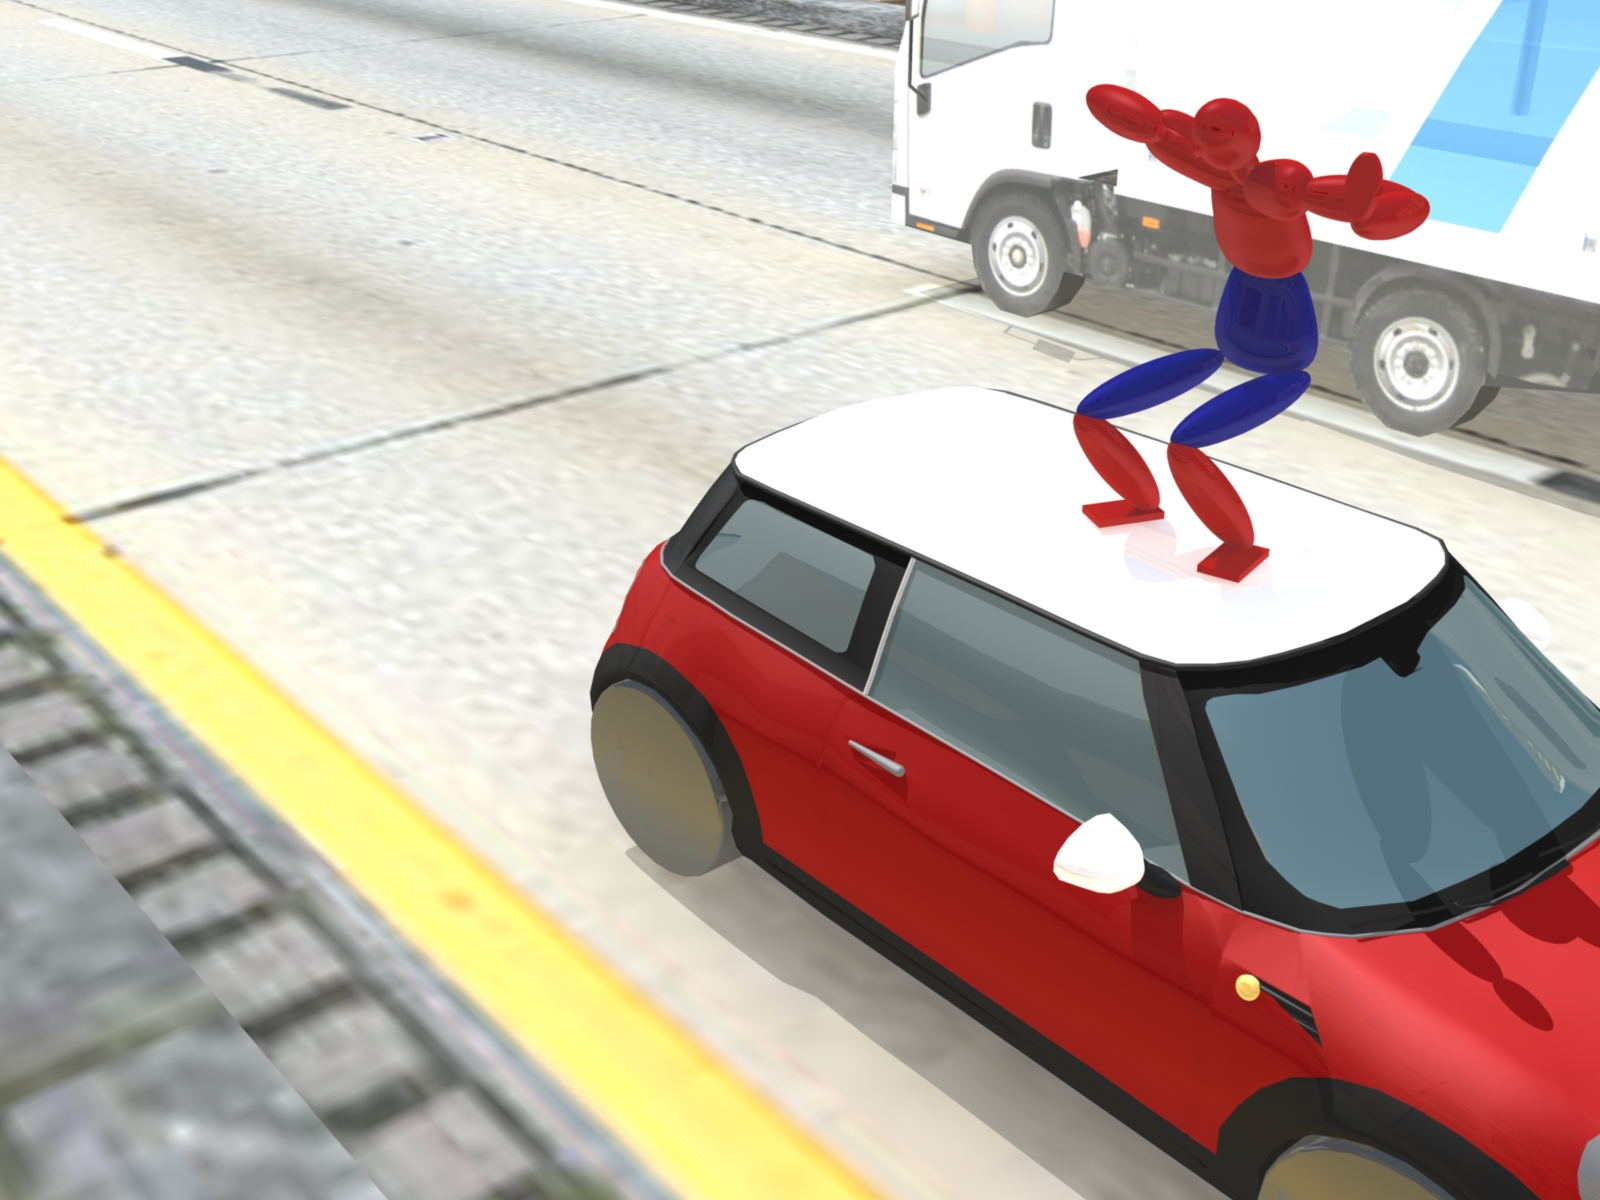
\includegraphics[width=0.48\textwidth]{images/intro_landing.jpg}
  \end{center}
   \vspace{-25pt}
  \caption{A falling motion of Parkour.}
  \label{fig:intro_landing}
   \vspace{-10pt}
\end{wrapfigure}

Inspired by falling skills of Parkour(\figref{intro_landing}), 
I formulate the falling problem
with three phases, \emph{airborne}, \emph{impact}, and \emph{rolling}
based on the contact states of a virtual character.
First, two sub-controllers are designed for the \emph{airborne} and
\emph{rolling} phases and a regression analysis is conducted to find 
an optimal landing angle that can connect two sub controllers at the
\emph{impact} phase.
I will demonstrate that the motion generated by the proposed controller
looks natural and induces smaller joint stress, which is still four times lower
than a uncontrolled rag-doll motion.



\subsection{Multiple Contact Planning for Humanoid falls}
\begin{wrapfigure}{l}{0.5\textwidth}
 \vspace{-25pt}
  \begin{center}
    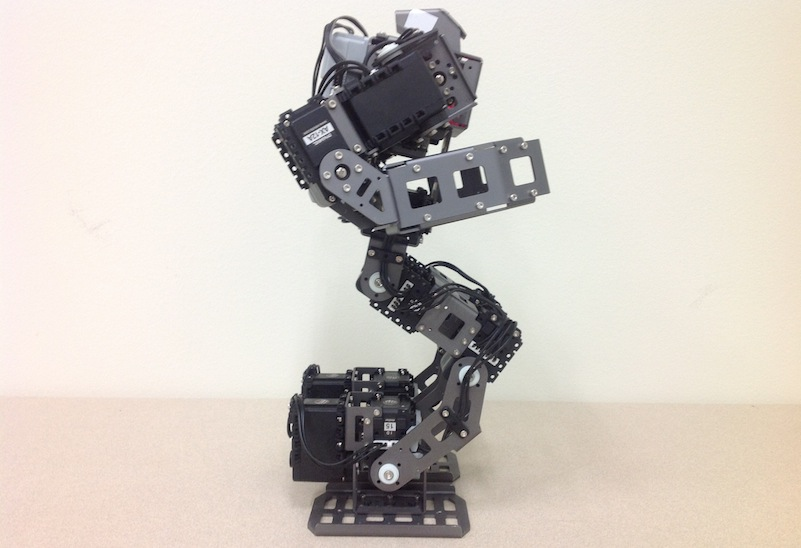
\includegraphics[width=0.48\textwidth]{images/intro_hardware.jpg}
  \end{center}
   \vspace{-25pt}
  \caption{Hardware of BioloidGP robot.}
   \vspace{-10pt}
  \label{fig:intro_hardware}
\end{wrapfigure}
% Goal, Method (Strength), Verification + Image
Chapter 4 will describe a robust falling strategy which plans for appropriate 
responses to a wide variety of falls, from a single step to recover a gentle
nudge, to a rolling motion to break a high-speed fall.
Our key observation is that  many existing falling techniques [Wang,Yun,Ukemi]
assume specific sequences of contacts and aim to break specific ranges of
falls and requires us to an additional decision layer to choose the best
falling strategy to the given state.
Instead, our multiple contact planning algorithm provides a unified framework
for various existing falling strategies, which can adjust the number and order
of contact sequences with respect to different magnitudes of perturbations.
In the proposed continuous space of strategies, our algorithm can efficiently
find the best falling strategy for the given initial state using a simplified
model and dynamic  programming.
To verify our framework, a variety of scenarios are tested on simulated
humanoids and the actual hardware (\figref{intro_hardware}) to show that our
algorithm plans versatile falling strategies with different contact sequences.

\section{Learning of Dynamic Controller for Characters}
% Introduction on the learning - Motivation, Description, Goal
Unlikely well-defined tasks such as reaching or walking,
agile motions cover a wide range of diverse skills such as vaulting, flipping,
or rolling.
Because these agile motions are governed by different mechanisms and
principles, manually designing and fine-tuning specialized controllers for all
tasks is not a practical approach.
Design of an individual physics-based controller for a new motor skill is 
a time-consuming task  which requires a lot of manual efforts from the controller
designer, from the design of the control mechanism to the tweaking of low-level
control parameters. 
To simplify the costly learning process, I will introduce an intuitive and 
interactive framework for developing controllers that is inspired by
how humans learn dynamic motor skills through a iterative process of coaching
and practicing.
Another important component for the iterative controller design process
is an efficient optimization to reduce a turn-around time.
In this purpose, we propose two optimization techniques that can extend the
popular policy search algorithm, CMA-ES, to accelerate the convergence rate
and to optimize a parametrized objective function.

\subsection{Iterative Design of Dynamic Controllers}
% Goal, Method (Strength), Verification + Image
\begin{wrapfigure}{r}{0.6\textwidth}
 \vspace{-10pt}
  \begin{center}
    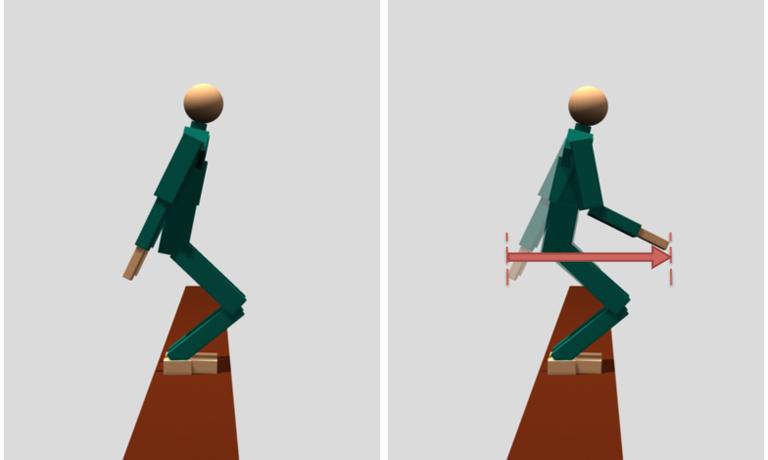
\includegraphics[width=0.58\textwidth]{images/intro_teach.png}
  \end{center}
   \vspace{-25pt}
  \caption{The proposed learning frame uses human readable instructions
    to teach motions.}
  \label{fig:intro_teach}
   \vspace{-10pt}
\end{wrapfigure}

In Chapter 5, we will describe an iterative framework to design dynamic
controllers using high-level, human-readable instructions,
inspired by a training process of athletes that consists of
interactive coaching and repetitive practices (\figref{intro_teach})
To enable interactive coaching, we introduce ``control rigs'' as
an intermediate layer of control module which allows more coordinated control
of the low level control variables and and provides more intuitive mapping to
high-level human instructions. 
During the practicing stage, control parameters are efficiently determined
using CMA-ES, which will be further improved in the following chapters.
The details of controllers development process using our iterative learning
framework will be shown with example iterative training procedures of parkour
motions.

\subsection{Optimization with Failure Learning}
% Goal, Method (Strength), Verification + Image
In Chapter 6, I will describe a new optimization algorithm for
highly-constrained problems.
A controller with many constraints is difficult to be optimized due to the
relatively small feasible regions with many local minima.
Our key idea comes from human’s ability to learn from failure. 
Because failure in the real world is usually associated with pain or injury,
humans tend to be very effective in characterizing the cause of failure and
trying to avoid the same mistakes in the future. 
Under the concept of ``learning from failure'', The proposed algorithm CMA-C
(Covariance Matrix Adaptation with Classification) utilizes the failed
simulation trials to approximate an infeasible region in the space of control
rig parameters so that it can predict validities of newly generated samples,
resulting a faster convergence than the standard CMA-ES.

\subsection{Optimization for Parametrized Motor Skills}
% Goal, Method (Strength), Verification + Image
In Chapter 7, I will explain an evolutionary optimization algorithm for
learning parameterized skills to achieve whole-body dynamic tasks.
The parametrization of the learned motor skills is an essential ability
because a robot can reinterpret the skill to a new situation, without
learning the entire motor skill from scratch.
Instead of maintaining a single Gaussian distribution, 
the algorithm reduces the number of samples by evolving a parametrized
probability distribution which describes a mapping from a task parameter
to the optimal control parameters.
I will test the proposed optimization algorithm for learning three parametrized
dynamic motor skills on a simulated humanoid robot, including jumping,
kicking, and walking. 

\section{Model-based Learning for Virtual and Real Characters}
% Goal, Method (Strength), Verification + Images
\begin{wrapfigure}{l}{0.5\textwidth}
 \vspace{-10pt}
  \begin{center}
    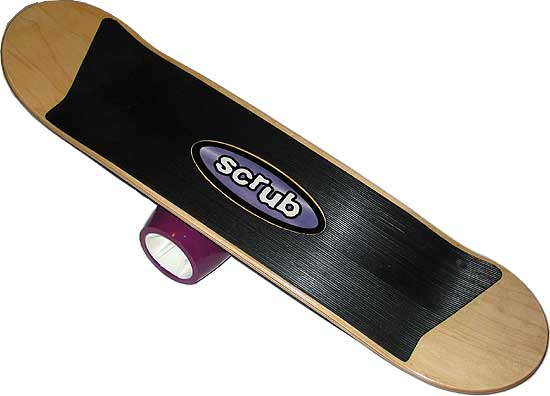
\includegraphics[width=0.48\textwidth]{images/intro_bongo.jpg}
  \end{center}
   \vspace{-25pt}
  \caption{Bongo Board balance toy.}
  \label{fig:intro_bongo}
   \vspace{-10pt}
\end{wrapfigure}

In Chapter 8, I will describe an iterative approach for for learning 
hardware models and optimizing control policies, which is designed for
reducing the number of expensive hardware experiments.
Computer simulation is often used to replace hardware experiments,
but it is difficult to obtain accurate simulation models and
simulation-optimized control policies are not likely to work on hardware.
To fill the gap between two system, we propose an algorithm for learning
hardware models and optimizing policies. 
Instead of learning hardware models from scratch, the proposed approach only
learns the difference from a simulation model using Gaussian 
As a proof of concept, I will validate the algorithm on two different 
simulation models, one with perfect contacts and one with realistic contacts,
by finding a balancing controller for a simple bipedal robot on a bongo board
(\figref{intro_bongo}).

\section{Contributions}
The control and optimization methods discussed in this dissertation provide
several contributions to the computer animation and robotics community. 
These contributions are as follows:

\begin{itemize}
\item \textbf{A falling and landing strategy for virtual characters}
  The falling strategy presented in the dissertation generates a natural falling
  and landing motion that falls from a wide range of heights and initial
  speeds, continuously rolls on the ground, and gets back on its feet without
  inducing large stress on joints at any moment.
\item \textbf{A multiple contact falling strategy for robots}
  We introduce a falling strategy for humanoid robots which can break a
  fall with minimal damage to the body parts by optimizing the number and
  locations of contacts for the given initial state. 
\item \textbf{An iterative learning framework for dynamic motor skills}
  We propose an iterative and interactive learning framework 
  using human readable instructions that can teach a variety of agile motions
  to virtual characters.
  Starting from a basic controller, the proposed framework allows a user 
  to easily train complex physics-based controllers 
  with only intuitive high-level instructions from the user.
\item \textbf{An optimization technique for highly constrained problems}
  We introduce a novel efficient optimization algorithm, CMA-C, that is 
  designed for the problem with many constraints and smaller feasible regions.
  The algorithm converges faster than the standard CMA-ES,
  by approximating the infeasible region using learned classifiers.
\item \textbf{An optimization technique for parametrized tasks}
  We introduce an efficient evolutionary optimization algorithm for learning
  parametrized whole-body dynamic tasks.
  By evolving parameterized sample distributions, our algorithm
  converges faster than the baseline algorithm, CMA-ES.
\item \textbf{A model-based policy search for reducing hardware experiments}
  We propose an iterative approach for learning hardware model and optimizing
  policies with as few hardware experiments as possible by learning
  \emph{dynamics bias}, which is difference between simulation and hardware
  models. 
\end{itemize}

\rule{0.95\textwidth}{1pt}

In the next chapter, I will discuss the related work conducted by other
researchers to address similar problems.

